\newpage
\subsection{QuizziPedia::Front-End::Controllers}

\begin{figure} [ht]
	\centering
	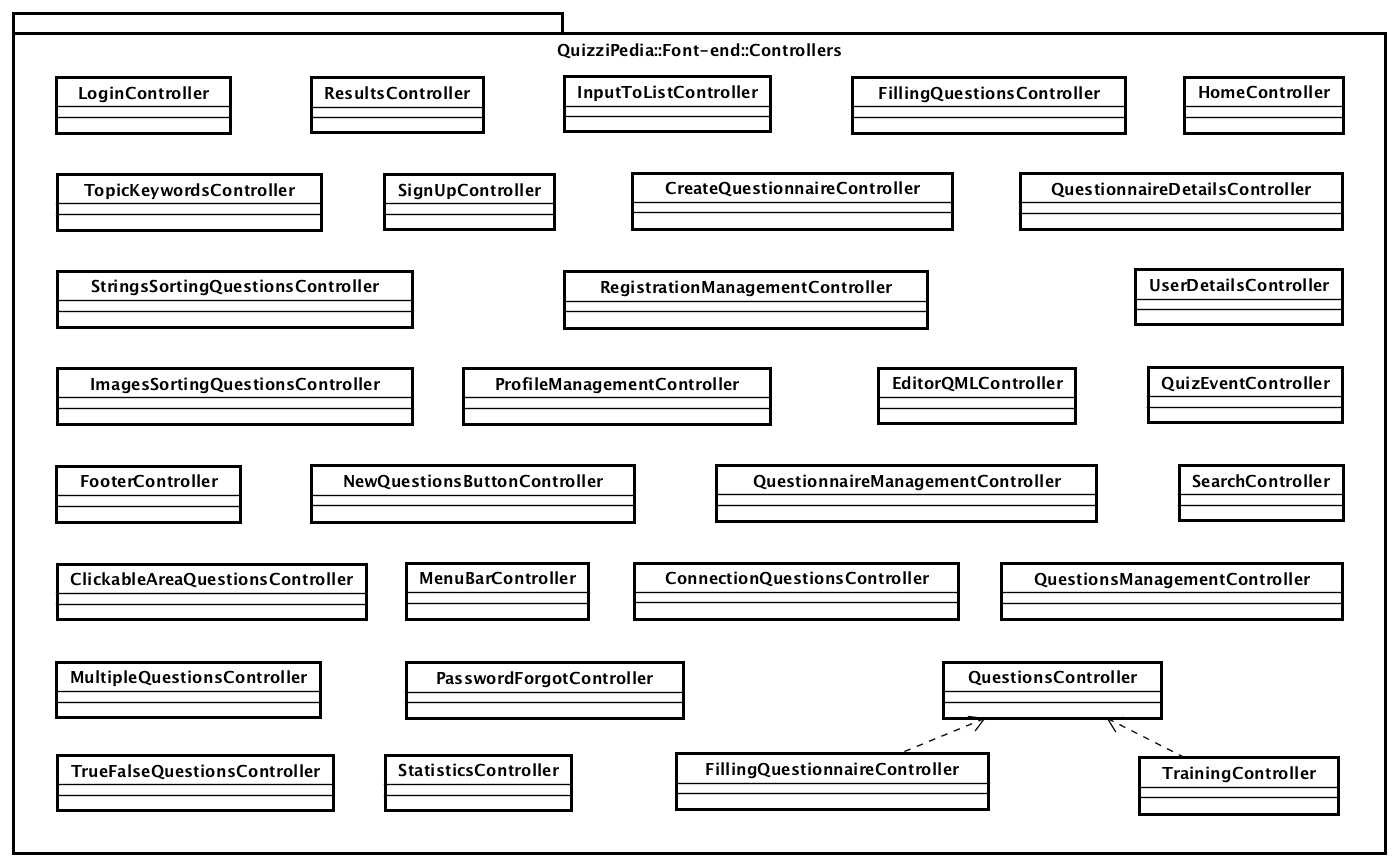
\includegraphics[scale=0.42]{UML/Package/QuizziPedia_Front-End_Controllers.png}
	\caption{QuizziPedia::Front-End::Controllers}
\end{figure} \FloatBarrier

\subsubsection{Informazioni generali}
\begin{itemize}
	\item \textbf{Descrizione}: \textit{package\ped{G}} che contiene i controller individuati per la parte front-end dell'applicazione;
	\item \textbf{Padre}: \texttt{Front-End};
	\item \textbf{Interazione con altri componenti}:
	\begin{itemize}
		\item \texttt{Models}: \textit{package\ped{G}} che contiene le classi model individuate;
		\item \texttt{Services}: \textit{package\ped{G}} che contiene le classi services individuate.
	\end{itemize}
	\item \textbf{Classi contenute}:
	\begin{itemize}
		\item \texttt{ClickableAreaQuestionController}: questa classe permette di gestire la creazione e la modifica di una domanda ad area cliccabile;
		\item \texttt{ConnectionQuestionController}: questa classe permette di gestire la creazione e la modifica di una domanda a collegamento;
		\item \texttt{CreateQuesrtionnaireController}: questa classe permette di gestire la creazione di un questionario;
		\item \texttt{EditorQMLController}: questa classe permette di gestire la creazione e la modifica di domande create tramite editor \textit{QML\ped{G}};
		\item \texttt{FillingQuestionnaireController}: questa classe permette di gestire la compilazione del questionario;
		\item \texttt{FillingQuestionsController}: questa classe permette di gestire la creazione e la modifica di una domanda	a riempimento di spazi;
		\item \texttt{HomeController}: questa classe permette di gestire la home page;
		\item \texttt{ImagesSortingQuestionsController}: questa classe permette di gestire la creazione e la modifica di una domanda a ordinamento immagini;
		\item \texttt{InputToListController}: questa classe permette di gestire l'inserimento di una lista di risposte durante la creazione di una domanda;
		\item \texttt{LoginController}: questa classe permette di gestire l'autenticazione dell'utente al sistema;
		\item \texttt{MenuBarController}: questa classe permette di gestire il menù fisso per ogni pagina;
		\item \texttt{MultipleQuestionController}: questa classe permette di gestire la creazione e la modifica di una domanda a risposta multipla;
		\item \texttt{NewQuestionButtonController}: questa classe permette di effettuare il redirect alla pagina di creazione nuova domanda;
		\item \texttt{PasswordForgotController}: questa classe permette di gestire il ripristino della password dimenticata;
		\item \texttt{ProfileManagementController}: questa classe permette di gestire il profilo personale di un utente;
		\item \texttt{QuestionnaireDeatailsController}: questa classe permette di gestire i dettagli di un questionario;
		\item \texttt{QuestionnaireManagementController}: questa classe permette di gestire tutti i questionari creati da un utente;
		\item \texttt{QuestionsController}: questa classe permette di gestire il recupero delle domande per far si che possano essere visualizzate nella modalità allenamento e nella compilazione dei questionari;
		\item \texttt{QuestionsManagementController}: questa classe permette di gestire le domande create dall'utente e di crearne di nuove;
		\item \texttt{QuizEventController}: questa classe permette di reagire ai comandi dell'utente durante la gestione dei suoi questionari;
		\item \texttt{RegistrationManagementController}: questa classe permette di gestire le iscrizione degli utenti ai questionari;
		\item \texttt{ResultQuestionnaireController}: questa classe permette di gestire la visualizzazione dei risultati di un singolo questionario;
		\item \texttt{SearchController}: questa classe permette di gestire la ricerca di questionari e utenti all'interno dell'applicazione;
		\item \texttt{SignUpController}: questa classe permette di gestire la registrazione di un utente al sistema;
		\item \texttt{StatisticsController}: questa classe permette di gestire le statistiche di un utente;
		\item \texttt{StringsSortingQuestionController}: questa classe permette di gestire la creazione e la modifica di una domanda a ordinamento di stringhe;
		\item \texttt{TopicKeywordsController}: questa classe permette di gestire il recupero delle parole chiave di un questionario;
		\item \texttt{TrainingController}: questa classe permette di gestire la modalità allenamento sottoponendo all'utente le giuste domande adatte al suo livello;
		\item \texttt{TrueFalseQuestionController}: questa classe permette di gestire la creazione e la modifica di una domanda	vero/falso;
		\item \texttt{UserDetailsController}: questa classe permette di gestire i dati di un utente da mostrare nella pagina di un profilo.
	\end{itemize} 
\end{itemize}